\documentclass{article}
\usepackage{graphicx} % Required for inserting images
\usepackage{hyperref}
\title{Homework 1 – Machine Learning (CS4342, Whitehill, C-Term 2025)}
\author{Artem Frenk and Daniel Gorbunov}
\date{January 29, 2025}

\begin{document}

\maketitle

\section{Question 4}
\begin{tabular}{|c|c|c|}
     \hline
     \texttt{n} & \texttt{trainingAccuracy} &\texttt{testingAccuracy}\\
     \hline
     400 & 0.8425 & 0.7112\\
     \hline
     600 & 0.8300 & 0.7500\\
     \hline 
     800 & 0.8075 & 0.7062\\
     \hline 
     1000 & 0.8200 & 0.7451\\
     \hline 
     1200 & 0.8042 & 0.7560\\
     \hline 
     1400 & 0.8021 & 0.7577\\
     \hline
     1600 & 0.7963 & 0.7681 \\
     \hline
     1800 & 0.7900 & 0.7609\\
     \hline 
     2000 & 0.7840 & 0.7648\\
     \hline 
     
\end{tabular} \\

As is apparent in the provided table, and this plot \ref{fig:convergence}, as the number of features $n$ is increased, the difference between the training and testing accuracy is decreased.  In addition, as the testing accuracy increases, the training accuracy decreases. However, at 800 training examples, there is a significant outlier, which is likely a result of the greedy algorithm selecting unoptimal pixel-pair locations. 
\begin{figure}
    \centering
    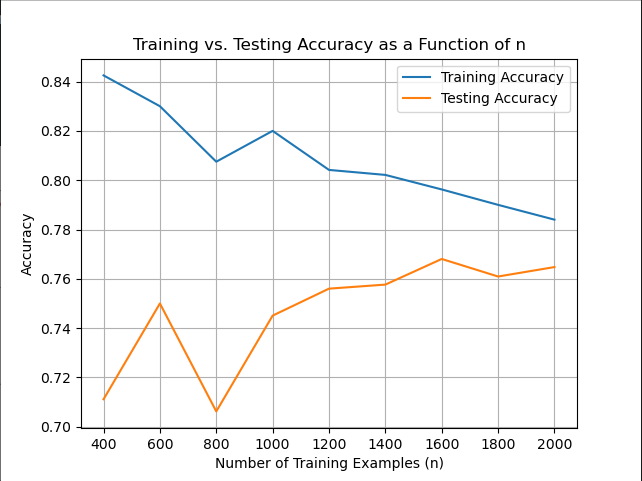
\includegraphics[width=1\linewidth]{Convergence.png}
    \label{fig:convergence}
\end{figure}
\section{Question 5}
\ref{fig:facepreds}
\begin{figure}
    \centering
    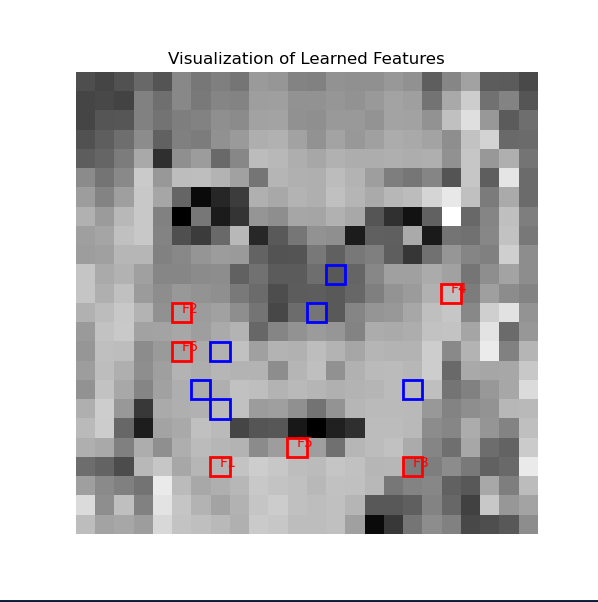
\includegraphics[width=1\linewidth]{FacePreds.png}
    \label{fig:facepreds}
\end{figure}

\end{document}
